\section{High energy physics research at the CMS 
     experiment at the Large Hadron Collider}


The Large Hadron Collider (LHC) is a gigantic scientific machine 
constructed 
below ground at the CERN Laboratory near Geneva, Switzerland, 
that is built to help answering unresolved fundamental questions in 
particle physics. 
Despite that the standard model (SM) of the particle physics has been 
tested 
to exquisite precision, it is considered to be an effective theory up to 
scale of about 1 TeV. 
One of the main goals for the LHC is to elucidate the nature of the 
electroweak symmetry
breaking mechanism, for which the Higgs mechanism is presumed responsible. 
With the discovery of a new particle consistent with the Higgs boson the 
LHC reached an important milestone.
The Higgs boson completes the table of the fundamental particles predicted
in the standard model. Now the LHC launches a large physics program 
dedicated 
to studying properties of a new observed boson that could shed a light on 
the origin
of mass.

In addition, there are mathematical inconsistencies in the SM at energy 
scales above about 1 TeV. These inconsistencies might be resolved by 
extensions of the SM, which could take the form 
of supersymmetry or extra dimensions, or might require invoking new forces 
and 
constituents. Hence there are many compelling reasons to investigate the 
TeV energy scale.
%There is a large effort in the physics community at the LHC targeting 
%searches for new physics. 


The Large Hadron Collider is the world's most powerful accelerator
built to explore the new energy domain.  It consists of the
27-kilometers ring of superconducting magnets that are designed to
direct and accelerate the proton beams up to an energy of 7 TeV each
(the LHC is presently operating at 3.5 TeV per beam). Prior to being
injected into the LHC ring protons pass a chain of smaller
pre-accelerators, each providing approximately 20-fold increase in the
proton energy.
%Once injected into the LHC ring two beams travel in opposite directions 
%in separate beam 
%pipes that are kept at ultrahigh vacuum of about $10^{-10}$ mbar. 
%Thousands of superconducting magnets of different  types are located 
%intermittently along the beam pipe.
%These superconducting magnets include 1232 dipole magnets of 15 m in 
%length, which provide a strong magnetic 
%field up to 8.3 T used to bend the beams, and 392 quadrupole magnets, 
%each 5-7 m long, used to focus the beams. 
%Eight radio frequency (RF) resonating cavities are responsible for 
%accelerating the beams through a field
%gradient of 5.5 MV/m and increasing the proton energy up to by 16 MeV per 
%turn. 
%Another type of magnet is used to squeeze the particles closer together 
%to increase the chances of collisions.
%Superconducting electromagnets are chilled by the super-fluid Helium II, 
%operated at temperature of 1.9 K. 
%At these temperatures the coils of electric cable made of the 
%niobium-titanium alloy operate in a superconducting state, efficiently 
%conducting electricity without resistance or loss of energy.
The proton beams consist of separate bunches of particles with about $1.4 
\times 10^{11}$ 
protons her bunch, and a time spacing of 50 ns, leading to a bunch 
crossing frequency of 20 MHz. 
%The time spacing is projected to be reduced to 25 ns in the future.
%The bunch pattern is formed in the 26 GeV Proton Synchrotron, and 
%determined by the injection scheme.
%The various gaps between bunches are required for synchronization, 
%acquiring of calibration data and providing
%resets to front-end electronics. 

The important characteristic of the machine is the instantaneous 
luminosity of the collisions
%, that is determined 
%based on the number of bunches per beam, the number of protons per bunch, 
%and other properties 
%of the machine, such as the transverse size of the beams at the 
%interaction point, the crossing angle 
%of the two colliding beams and the beam emittance.
that reflects how well each beam is focused, and how well the
beams are aimed at each other to produce proton-proton collisions.
During 2012 at the peak performance the LHC operated at the highest
luminosities ever achieved at hadron colliders, of up 
to ${\cal L} = 7 \cdot 10^{33} \,\mathrm{cm}^{-2}\, \mathrm{s}^{-1}$ with 
4 TeV energy per beam, and is expected to achieve the design luminosity 
${\cal L} = 10^{34} \,\mathrm{cm}^{-2} \,\mathrm{s}^{-1}$, and the design 
energy per beam of 7 TeV
after the long shutdown (LS1) of 2013-2014. At these luminosities 
the high proton bunch density combined with the strong focusing at the 
interaction point also results 
in about 40 inelastic $pp$ interactions per bunch crossing, referred to as 
``pile-up". 

The beams inside the LHC are made to collide at four locations around the 
accelerator ring, corresponding 
to the positions of the particle detectors, situated in four underground 
caverns. These include two large 
general-purpose detectors CMS and ATLAS, and two medium-size specialized 
experiments ALICE and LHCb.

The Compact Muon Solenoid (CMS) detector is one of the two large 
multi-purpose detectors 
installed at opposite sides of the LHC accelerator ring (see Figure~\ref{fig:SiPix}). 
The CMS is an azimuthally and forward-backward symmetric 
detector designed to study $pp$ reactions at the LHC.
The characteristic feature of the CMS detector is the superconducting
solenoid, 6 m in diameter and 13 m in length, and 10,000 tons in mass, 
which provides an axial magnetic field of 3.8~T. 
%A total of 19.5 kA electrical current flows through 
%superconducting cables cooled by liquid Helium down to 4.6 K.
%The stored energy of the magnetic field is about 2.7 GJ.
%The iron return yoke is provided by five barrel rings around the coil and 
%three endcap discs on each side. 
The strong magnetic field allows to achieve a large bending power and good 
momentum resolution of the charged particles within a compact 
spectrometer. 
Outside the magnet coil %and inside the iron return yoke 
is installed the muon system, that 
is designed to provide a highly reliable muon identification, and
improve the muon momentum resolution for high-momentum muons. 
%This is achieved by extrapolating 
%the muon trajectory beyond the return yoke back to the beamline.
%The return magnetic field is large enough
%to saturate 1.5 m of iron, allowing 4 muon stations to be integrated to 
%ensure robustness
%and full geometric coverage. Each muon station consists of several layers 
%of alluminium drift
%tubes (DT) in the barrel region ($|\eta| < 1.2$),
% and cathode strip chambers (CSCs) in the endcap region 
%($1.2 < |\eta| < 2.4$),
%complemented by resistive plate chambers (RPCs) in 
%both the barrel and the endcap. The RPCs 
%and are operated in avalanche mode to ensure a fast response 
%with good time resolution, 
%but with a coarser position resolution than the DTs or CSCs.

The bore of the magnet coil accommodates the inner tracker and the
calorimetry inside. 
The electromagnetic calorimeter (ECAL) with an inner radius of 129 cm
is used to measure electrons and photons in the region $|\eta| < 3.0$.
The ECAL makes use of lead tungstate (PbWO4) crystals, which 
provide an excellent energy resolution. 
%They have short radiation
%($X_0 = 0.89$ cm) and Moliere (2.2 cm) lengths, that allowed a design of 
%compact calorimeter.
%The crystals are fast (80\% of the light is emitted within 25 ns) and 
%radiation resistant. 
%The scintillation light is detected by photodetectors with intrinsic gain 
%that can operate in a magnetic field.
%Silicon avalanche
%photodiodes are used in the barrel region and vacuum phototriodes in the 
%endcap region. 
Preshower detectors are mounted in front of the endcap ECAL and are used 
to help in the identification 
of neutral pions.

Jet energies are measured with the hadron calorimeter (HCAL),
%, which
%is mainly located inside of the magnet coil and 
that surrounds 
the ECAL system completely covering the pseudorapidity range of $|\eta| < 
3.0$.
The HCAL uses brass as an absorber material, which is interlayed with 
plastic 
scintillator tiles.
%
%Its design is strongly constrained by the choice of magnet parameters. 
%To maximize the amount of material fitted into the solenoid magnet, 
%brass is chosen as an absorber material, as it is non-magnetic and has a 
%reasonably short interaction length.
%The amount of space devoted to the active medium is minimized
%by using plastic scintillator tiles 3.7 mm thick 
%with embedded wavelength-shifting fibres that convert and transmit 
%the scintillation light to multi-channel hybrid photodiode detectors. 
%The scintillator tiles are interlayed and bolted together with flat 5 cm 
%thick brass absorber plates.
The overall assembly has essentially no uninstrumented regions or dead 
areas, which provide 
a good hermicity of the detector for the transverse missing energy 
measurement.
To improve the energy resolution an additional layer of scintillators
%, referred to as the 
%hadron outer (HO) detector, 
placed outside of the coil.
%The inclusion of the HO extends the total depth of the HCAL from 5.8 to 
%11.0 interaction lengths
%in the central region.
 
 The innermost part of the CMS detector is the silicon tracking system.
It consists of two sub-detectors: the silicon pixel detector, located 
closest to the interaction 
 region, and the silicon strip detector, that provide a high precision 
measurement of the trajectories
 of charged particles in the region of $|\eta| < 2.5$.
 In the central part of the CMS detector, the silicon microstrip detectors 
are placed 
 at radii between 20 and 110 cm, and overall 
 consist of 10 layers, some of which
% separated into an Inner and an Outer Barrel. 
% The Inner Barrel is made of 4 layers covering the region $|z| < 65$ cm, 
% and
%% using 320 $\mu$m silicon sensors and 80-120 $\mu$m strip pitch.
% the Outer Barrel comprises 6 layers with a half-length of $|z| < 110$ cm
% %with thicker silicon sensors (500 $\mu$m) and a larger strip pitch 
%(120-180 $\mu$m).
% Some of the layers of both the Inner and Outer Barrels 
are made with stereo modules, 
 %The first two layers of Inner and Outer Barrels 
 %are made with stereo modules with a stereo angle of 100 mrad in order 
 %The strip tracker barrel detector provides 
 so that the track trajectory is measured in 
 %a measurement in 
 both $r-\phi$ and $r-z$ coordinates.
 The strip tracker endcaps consist of 9 large disks on each end
 %that extend into the region 120 cm $ < |z| < $ 280 cm, 
 and 
 3 small disks that fill the gaps between the barrel and the tracker 
endcaps.
 %The endcap modules are arranged in rings, centered on the beam lime, 
 %with strips 
 %that point towards the beam line. 
  In total the silicon strip tracker has 9.6 million strips and 198 m$^2$
of active silicon area, and it is the largest silicon tracker ever built.

The pixel detector  is the centerpiece of the CMS silicon tracker system 
(see Figure~\ref{fig:SiPix}), 
and is the subject of this proposal.
It provides three high-precision space point measurements for 
reconstruction of charged particle trajectories. 
With close proximity to the interaction point (4.4 cm) it plays a key role 
in the robust identification of 
primary vertices and reconstruction of secondary vertices essential for 
the highly efficient identification 
of long-lived particles, such as $b$ quarks. 
 
The silicon detector comprises 66 million pixels with dimensions of 100 
$\mu$m by 150 $\mu$m.
These are arranged in three cylindric layers in the barrel region (BPIX) 
covering $|\eta| < 2.2$ 
and two endcap disks (FPIX)  at each side of the detector, perpendicular 
to the beam axis, and covering $2.2 < |\eta| < 2.5$.
% as shown in Figure~\ref{fig:SiPix}.
The barrel layers are installed at radii of 4.4 cm, 7.3 cm, and 10.2 cm 
from 
the beam axis. The endcaps are found at $z$-positions of 32.5 cm and 46.5 cm, and 
cover the region 
between 6 cm and 15 cm from the beam axis. 
The inner pixel layers are exposed to a radiation fluence as high as 
$3\times 10^{14} \,\mathrm{cm}^{-2} $ 
per year, requiring a detector and electronics of radiation-hard design. 
This is achieved by using deep sub-micron CMOS technology.

%
%\begin{figure}[htb]
%  \centering
%  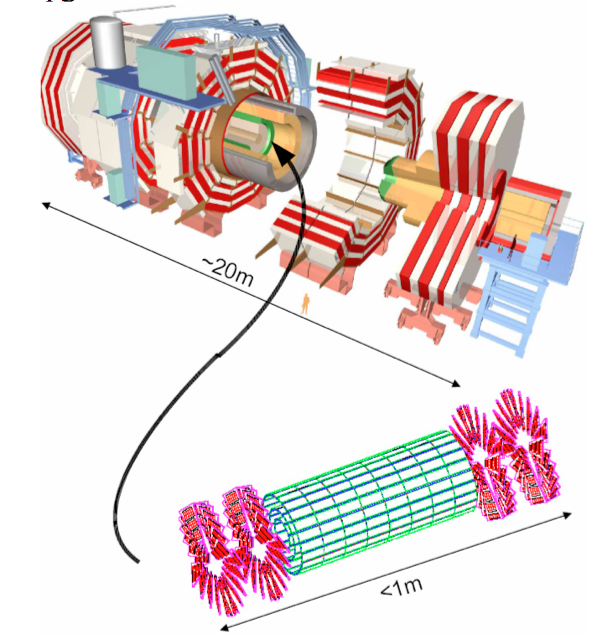
\includegraphics[width=0.5\textwidth]{CMS_detector_low_res.png}
%  \caption{\label{fig:cms}
%    A diagram of the CMS experiment and the pixel portion of the
%    tracking detector.
%  }
%\end{figure}
%
\begin{figure}[htb]
  \centering
  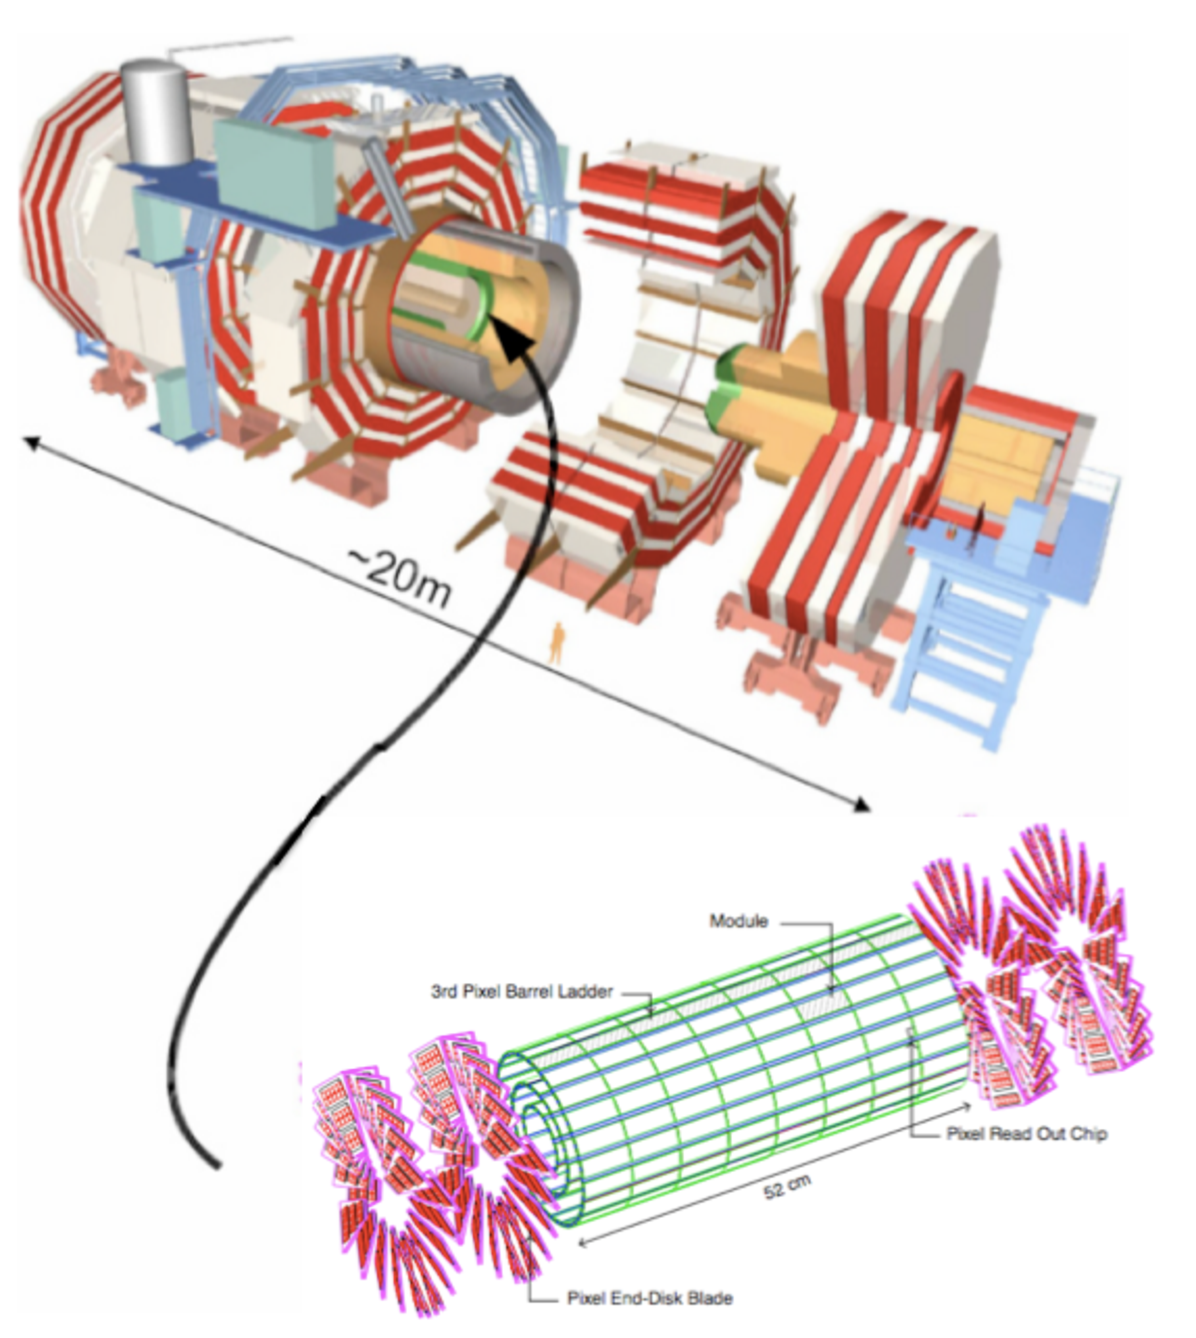
\includegraphics[width=0.5\textwidth]{CMSnSiPix.pdf}
  \caption{\label{fig:SiPix}
  A diagram of the CMS experiment and the pixel portion of the tracking 
detector.
  %The CMS pixel detector in the current configuration. 
  The pixel barrel expands to $\pm26$ cm. A ladder of eight modules is 
highlighted. Each
module is made of 16 ROCs. 
  }
\end{figure}


The barrel detector consists of 768 pixel modules arranged into 
half-ladders of 4 identical modules
each. The $r-\phi$ resolution is improved via the charge sharing between 
pixels due to 
the large Lorentz angle (23$^\circ$).
The endcap disks are assembled in a turbine-like geometry with blades 
rotated by 20$^\circ$
and also benefit from the Lorentz effect. The endcap disks comprise 672 
pixel modules 
with 7 different modules in each blade.
The pixel detector is able to attain a spatial 
resolution of 10 $\mu$m in the $r-\phi$ and 20 $\mu$m in the $r-z$ 
coordinates, 
almost ten times smaller than the pixel size itself.

The LHC bunch crossing rate of 40 MHz results in $\approx 10^9$ 
interactions per second, 
requiring a rejection factor of order $10^6$ to reduce the rate to a level 
consistent 
with the possible rate of archiving data. The CMS trigger system achieves 
this in two stages. 
At the first stage, the Level-1 trigger system consisting of custom 
hardware processors,
makes a decision within 1 $\mu$s. 
Data collected by the various sub-detector components are held in buffers 
for longer period (3.2 $\mu$s)
required for the transit and reaching a decision for a particular bunch 
crossing. 
At the second stage the High-Level trigger (HLT) system 
runs more sophisticated reconstruction algorithms on a dedicated online 
computing farm. 
The reconstruction of tracks and vertices is made on this stage.
The Level-1 rate is limited to 100 kHz, and the HLT further reduces the 
Level-1 rate to 400 Hz 
for mass storage. These requirements pose constraints on the data 
acquisition system of the pixel 
detector.

In the pixel detector 
each pixel barrel module is read out by 16 Read-Out-Chips (ROCs)
bump-bonded to sensor arrays and 
arranged in $2\times8$ geometry.
In the endcaps due to the blade design the sensor area varies  in size 
from 2 to 10 ROCs per module.
The ROC uses a serial scheme to read an array of 52$\times$80 pixels in 
double columns.
A token bit manager chip (TBM) controls the readout scan of a group of 8 
to 16 readout chips.
The TBM also formats data packets and signals errors.  
Both the readout chip and TBM are designed in 0.25 $\mu$m bulk CMOS 
technology, 
providing the most radiation hard solution.
Due to a large number of pixels a full readout is impossible, and 
zero-suppression 
is implemented at a very early stage.
Only analog signals over threshold and corresponding pixel addresses are 
stored in a data buffer, 
waiting for the Level-1 trigger decision. 
A data packet is sent through each link for every triggered event, even if 
no pixels were hit.
In this case a packet includes a header and trailer provided by the TBM 
chip. 

Following a Level-1 trigger accept, data are transmitted through optical 
links to the readout 
electronics, Front-End-Drivers (FEDs), located in the counting room 100 m 
away from the detector. 
In addition to the analog pixel-charge amplitude several compressed 
digital signals, such 
as pixel and column addresses, ROC's IDs and trigger numbers are also 
transmitted. 
%In the barrel, groups of 8 to 16 ROCs are connected to one readout link, 
%whereas in the endcaps
%there are 21 or 24 ROCs per link. 
The 40 Pixel FED modules receive data packets, perform digitization and 
data formatting, 
and send them to the CMS data acquisition system.

The design concept of the CMS pixel detector accommodates relatively 
frequent access for 
replacement of silicon pixel layers.
%The pixel system is installed inside a cylindrical volume with a diameter 
%of 42 cm and 
%a length of 5.6 m formed by the inner wall of the CMS strip tracker. 
The whole pixel
system is split vertically and mounted on wheels, thus the complete
pixel detector can be extracted from the CMS core during long enough LHC downtimes.
It is foreseen that the first replacement of the full pixel detector will
happen during the Phase 1 Upgrade several years from now (see Section~\ref{sec:upgrade}),
and the IRES participants are expected to contribute to this upgrade project
(see Section~\ref{sec:projects}).

% guided by grooves in the 
%floor and ceiling 
%of the support tube. The barrel structure consists of the aluminum cooling 
%tubes connected
%by thin carbon fiber blades and attached to cooling manifolds embedded in 
%the bulkheads.
%The material of the pixel barrel amounts to 5 percent of a radiation 
%length in the central region.
%Sensors and read-out chips contribute one third of the material, while the 
%support structure
%and cooling fluid contribute about 50 percent.


